\documentclass[11pt, oneside]{article}   	% use "amsart" instead of "article" for AMSLaTeX format
\usepackage{geometry}                		% See geometry.pdf to learn the layout options. There are lots.
\geometry{letterpaper}                   		% ... or a4paper or a5paper or ... 
%\geometry{landscape}                		% Activate for for rotated page geometry
%\usepackage[parfill]{parskip}    		% Activate to begin paragraphs with an empty line rather than an indent
\usepackage{graphicx}				% Use pdf, png, jpg, or eps with pdflatex; use eps in DVI mode
								% TeX will automatically convert eps --> pdf in pdflatex		
\usepackage{amssymb}
\usepackage{amsmath}

\usepackage[numbered]{mcode}

\newcommand{\HRule}{\rule{\linewidth}{0.5mm}}

\title{A Birth-Death Process}
\setlength\parindent{0pt}

\begin{document}
\frenchspacing
\begin{titlepage}
		\begin{center}
			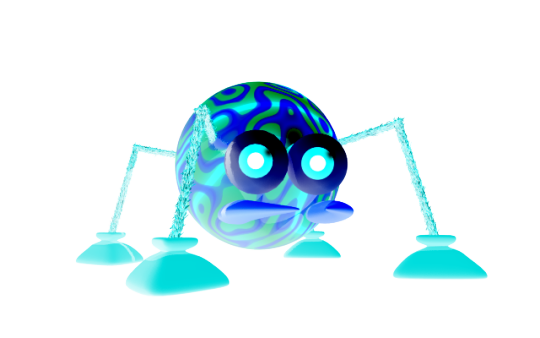
\includegraphics[scale=0.2]{logo}\\[1cm]
			
			\textsc{\LARGE MAT 485 Project 2}\\[2cm]
			\textsc{\Large Cal Poly Pomona}\\[1cm]
			
		
			\HRule \\[0.4cm]
			{\huge \bfseries A Two-Mass Oscillator \\[0.4cm]}
			\HRule \\[2cm]
			
			\noindent
			\begin{minipage}{0.4\textwidth}
				\begin{flushleft}
					\large
					\emph{Authors:}\\
					Morgan Rupard \\ Aaron Gaut
				\end{flushleft}
			\end{minipage}
			\begin{minipage}{0.4\textwidth}
				\begin{flushright}
					\large
					\emph{Professor:}\\
					Dr. Jennifer Switkes
			\end{flushright}
			\end{minipage}
			
			\vfill
			
			{\large March $7^{\text{th}}$, 2016}
		\end{center}
	\end{titlepage}

\tableofcontents
\newpage

\section{Introduction}

\end{document}  
